% \iffalse meta-comment
% A LaTeX Class for Semantic Lectures Slides (originally developed for Michael Kohlhase)
% Copyright (c) 2019 Michael Kohlhase, all rights reserved
%               this file is released under the
%               Gnu Library Public Licences (LGPL)
%
% The original of this file is in the public repository at 
% http://github.com/sLaTeX/sTeX/
% \fi
% 
% \iffalse
%
%<*driver>
\def\libfolder#1{../../lib/#1}
\RequirePackage{paralist}
\ifcsname stexdocpath\endcsname\else\def\stexdocpath{.}\fi
\documentclass[full]{l3doc}
%\RequirePackage{document-structure}
\usepackage[hyperref=auto,style=alphabetic]{biblatex}
\usepackage[mathhub=\stexdocpath/mh,usesms]{stex}
\usepackage{stex-highlighting,stexthm}

\newif\ifhadtitle\hadtitlefalse

\def\fileversion{3.3.0}
\def\filedate{\today}
\def\stexdoctitle#1#2{\title{#1\thanks{Version {\fileversion} (last revised {\filedate})} }\def\thispkg{#2}}

\author{Michael Kohlhase, Dennis Müller\\
 	FAU Erlangen-Nürnberg\\
 	\url{http://kwarc.info/}
}

\def\stexmaketitle{\ifhadtitle\else\hadtitletrue\maketitle\fi}

\def\docmodule{
\begin{document}
  \EnableManual
  \DisableImplementation
  \DocInput{\jobname.dtx}
  \EnableImplementation
  \DisableDocumentation
  \DisableManual
  \DocInputAgain
  \clearpage
  \PrintIndex
\end{document}
}

\ExplSyntaxOn
  \bool_new:N \g_stexdoc_typeset_manual_bool
  \NewDocumentCommand \EnableManual {}{
    \bool_gset_true:N \g_stexdoc_typeset_manual_bool
  }
  \NewDocumentCommand \DisableManual {}{
    \bool_gset_false:N \g_stexdoc_typeset_manual_bool
  }
  \NewDocumentEnvironment {stexmanual} {} {
    \bool_if:NTF \g_stexdoc_typeset_manual_bool
      {\bool_set_false:N \l__codedoc_in_implementation_bool}
      {\comment}
  }{
    \bool_if:NF \g_stexdoc_typeset_manual_bool {\endcomment}
  }
\ExplSyntaxOff

%\usepackage{makeidx}
%\makeindex

%\usepackage{document-structure}
\ExplSyntaxOn
\int_new:N \l_stex_docheader_sect

\cs_new_protected:Nn \stexdoc_do_section:n {
  \int_case:nnF \l_stex_docheader_sect {
    {0}{\cs_if_exist:NTF \part {\part{#1}}{
      \int_incr:N \l_stex_docheader_sect
      \stexdoc_do_section:
    }}
    {1}{\cs_if_exist:NTF \chapter {\chapter{#1}}{
      \int_incr:N \l_stex_docheader_sect
      \stexdoc_do_section:
    }}
    {2}{\section{#1}}
    {3}{\subsection{#1}}
    {4}{\subsubsection{#1}}
  }{\paragraph{#1}}
  \int_incr:N \l_stex_docheader_sect
}
%\int_incr:N \l_stex_docheader_sect
\NewDocumentEnvironment{sfragment}{m}{
  \stexdoc_do_section:n{#1}
}{}

\cs_set_nopar:Nn \_stexdoc_do_cs:Nn {
  \stex_debug:nn{here}{\tl_to_str:n{#1},~#2}
  \cs_if_exist:cTF{s\tl_to_str:n{#2}}{
    \cs_if_exist:cTF{s\tl_to_str:n{#2}name}{
    \symref{#2-sym}{#1{#2}}
    }{#1{#2}}
  }{
    #1{#2}
  }
}
\let\my_old_cs\cs
\protected\def\cs#1{
  \_stexdoc_do_cs:Nn \my_old_cs{#1}
}
\let\my_old_cmd\cmd
\protected\def\cmd#1{
  \_stexdoc_do_cs:Nn \my_old_cmd{#1}
}

\ExplSyntaxOff

\mhinput[sTeX/Documentation]{../lib/examples.tex}
\begin{document}
  \DocInput{\jobname.dtx}
\end{document}
%</driver>
% \fi
% 
% \GetFileInfo{notesslides.cls}
% \MakeShortVerb{\|}
%
% \def\twin#1#2{\index{#1!#2}\index{#2!#1}}
% \def\twintoo#1#2{{#1 #2}\twin{#1}{#2}}
% \def\atwin#1#2#3{\index{#1!#2!#3}\index{#3!#2 (#1)}}
% \def\atwintoo#1#2#3{{#1 #2 #3}\atwin{#1}{#2}{#3}}
%
% \def\scsys#1{{{\sc #1}}\index{#1@{\sc #1}}}
% \def\stex{\hbox{\raisebox{-.5ex}S\kern-.5ex\TeX}}
% \def\sTeX{\stex}
% \def\cnxml{\scshape{CNXml}}
% \def\connexions{\scshape{Connexions}}
% \def\element#1{{\ttfamily{#1}}}
% \def\snippet#1{{\ttfamily{#1}}}
% \def\cnxlatex{CNX\LaTeX\xspace}
% \def\mathml{{\scshape{MathML}}\xspace}
% \def\omdoc{OMDoc\xspace}
% \def\activemath{{\scshape{ActiveMath}}\xspace}
% \def\textwarning{
\includegraphics[width=1.2em]{stex-dangerous-bend}\xspace}
% 
% \title{NotesSlides -- Slides and Course Notes\thanks{Version {\fileversion}
% (last revised {\filedate})}}
%    \author{Michael Kohlhase\\
%            FAU Erlangen-N\"urnberg\\
%            \url{http://kwarc.info/kohlhase}}
% \maketitle
%
%\ifinfulldoc\else
% This is the documentation for the \pkg{notesslides} package.
% For a more high-level introduction, 
%  see \href{\basedocurl/manual.pdf}{the \sTeX Manual} or the
% \href{\basedocurl/stex.pdf}{full \sTeX documentation}.
%
% \begin{sfragment}{The User Interface}
% \begin{sfragment}{Introduction}
  The \pkg{notesslides} document class is derived from |beamer.cls|~\cite{beamerclass:on},
it adds a ``notes version'' for course notes that is more suited to printing than the one
supplied by |beamer.cls|.

The \pkg{notesslides} class takes the notion of a slide frame from Till Tantau's excellent
\pkg{beamer} class and adapts its notion of frames for use in the \sTeX and \OMDoc. To
support semantic course notes, it extends the notion of mixing frames and explanatory
text, but rather than treating the frames as images (or integrating their contents into
the flowing text), the \pkg{notesslides} package displays the slides as such in the course
notes to give students a visual anchor into the slide presentation in the course (and to
distinguish the different writing styles in slides and course notes).

In practice we want to generate two documents from the same source: the slides for
presentation in the lecture and the course notes as a narrative document for home
study. To achieve this, the \pkg{notesslides} class has two modes: \emph{slides mode} and
\emph{notes mode} which are determined by the package option. 
\end{sfragment}

\begin{sfragment}{Package Options}
  The \pkg{notesslides} class takes a variety of class options:

  \begin{variable}{slides,notes} The options |slides| and |notes| switch between slides
    mode and notes mode (see \sref{sec:user:notesslides}).
  \end{variable}

  \begin{variable}{sectocframes} If the option |sectocframes| is given, then for the
    |sfragment|s, special frames with the |sfragment| title (and number) are generated.
  \end{variable}

  \begin{variable}{frameimages,fiboxed}
    If the option |frameimages| is set, then slide mode also shows the
    |\frameimage|-generated frames (see \sref{sec:user:frameimage}). If also the |fiboxed|
    option is given, the slides are surrounded by a box.
  \end{variable}
\end{sfragment}

\begin{sfragment}[id=sec:user:notesslides]{Notes and Slides}

\begin{environment}{frame}
  Slides are represented with the |frame| environment just like in the \pkg{beamer} class,
  see~\cite{Tantau:ugbc} for details.
\end{environment}

\begin{environment}{note}
  The \pkg{notesslides} class adds the |note| environment for encapsulating the course
  note fragments.
\end{environment}
  
\begin{dangerbox}
  Note that it is essential to start and end the |notes| environment at the start of the
  line -- in particular, there may not be leading blanks -- else {\LaTeX} becomes confused
  and throws error messages that are difficult to decipher.
\end{dangerbox}

By interleaving the |frame| and |note| environments, we can build course notes as shown
here:

\begin{stexcode}
\ifnotes\maketitle\else
\frame[noframenumbering]\maketitle\fi

\begin{note}
  We start this course with ...
\end{note}

\begin{frame}
  \frametitle{The first slide}
  ...
\end{frame}
\begin{note}
  ... and more explanatory text
\end{note}

\begin{frame}
  \frametitle{The second slide}
  ...
\end{frame}
...
\end{stexcode}

\begin{function}{\ifnotes}
  Note the use of the |\ifnotes| conditional, which allows different treatment between
  |notes| and |slides| mode -- manually setting |\notestrue| or |\notesfalse| is strongly
  discouraged however.
\end{function}
 
\begin{dangerbox}
  We need to give the title frame the |noframenumbering| option so that the frame
  numbering is kept in sync between the slides and the course notes.
\end{dangerbox}

\begin{dangerbox}
  The \pkg{beamer} class recommends not to use the |allowframebreaks| option on frames
  (even though it is very convenient). This holds even more in the |notesslides| case: At
  least in conjunction with |\newpage|, frame numbering behaves funnily (we have tried to
  fix this, but who knows).
\end{dangerbox}
\end{sfragment}

\begin{function}{\inputref*}
  If we want to transclude a the contents of a file as a note, we can use a new variant
  |\inputref*| of the |\inputref| macro: |\inputref*{foo}| is equivalent to
  |\begin{note}\inputref{foo}\end{note}|.
\end{function}

\begin{environment}{nparagraph, nparagraph, ndefinition, nexample, nsproof, nassertion}
  There are some environments that tend to occur at the top-level of |note|
  environments. We make convenience versions of these: e.g. the |nparagraph| environment
  is just an |sparagraph| inside a |note| environment (but looks nicer in the source,
  since it avoids one level of source indenting). Similarly, we have the |nfragment|,
  |ndefinition|, |nexample|, |nsproof|, and |nassertion| environments.
\end{environment}

\begin{sfragment}{Customizing Header and Footer Lines}
  The \pkg{notesslides} package and class comes with a simple default theme named
  \pkg{sTeX} that provided by the \pkg{beamterthemesTeX}. It is assumed as the default
  theme for \sTeX-based notes and slides.
  The result in |notes| mode (which is like the |slides| version except that the slide
  hight is variable) is
  
  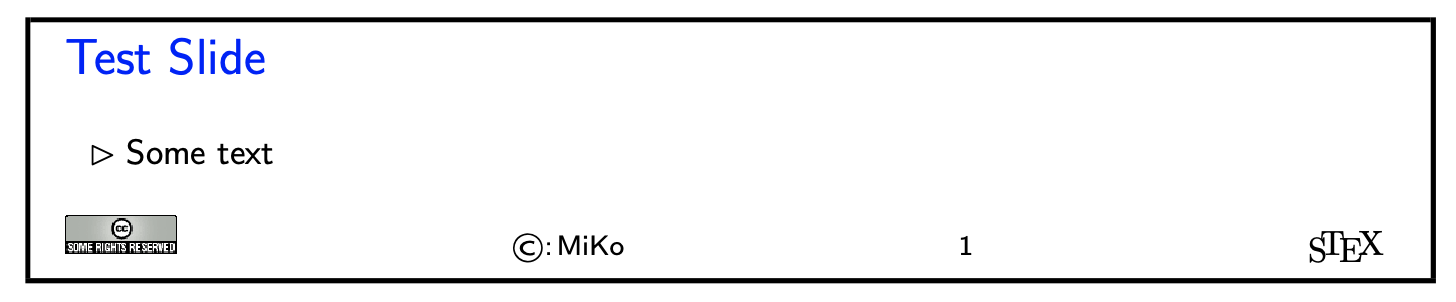
\includegraphics[width=.95\textwidth]{\stexdocpath/../lib/img/notes-frame}
  
The footer line can be customized. In particular the logos. 

\begin{function} {\setslidelogo}
  The default logo provided by the \pkg{notesslides} package is the {\sTeX} logo it can be
  customized using |\setslidelogo{|\meta{logo name}|}|.
\end{function}

\begin{function}{\setsource}
  The default footer line of the \pkg{notesslides} package mentions copyright and
  licensing. In \pkg{notesslides} |\source| stores the author's name as the copyright
  holder. By default it is the author's name as defined in the |\author| macro in the
  preamble.  |\setsource{|\meta{name}|}| can change the writer's name.
\end{function}

\begin{function}{\setlicensing}
  For licensing, we use the Creative Commons Attribuition-ShareAlike license by default to
  strengthen the public domain. If package |hyperref| is loaded, then we can attach a
  hyperlink to the license logo. |\setlicensing[|\meta{url}|]{|\meta{logo name}|}| is used
  for customization, where \meta{url} is optional.
\end{function}
\end{sfragment}

\begin{sfragment}[id=sec:user:frameimages]{Frame Images}
 Sometimes, we want to integrate slides as images after all -- e.g. because we already
have a PowerPoint presentation, to which we want to add \sTeX notes.

\begin{function}{\frameimage,\mhframeimage}
  In this case we can use |\frameimage[|\meta{opt}|]{|\meta{path}|}|, where \meta{opt} are
  the options of |\includegraphics| from the \pkg{graphicx} package~\cite{CarRah:tpp99}
  and \meta{path} is the file path (extension can be left off like in
  |\includegraphics|). We have added the |label| key that allows to give a frame label
  that can be referenced like a regular |beamer| frame.

The |\mhframeimage| macro is a variant of |\frameimage| with repository support. Instead
of writing
\begin{stexcode}
\frameimage{\MathHub{fooMH/bar/source/baz/foobar}}
\end{stexcode}
  we can simply write (assuming that |\MathHub| is defined as above)
\begin{stexcode}
\mhframeimage[fooMH/bar]{baz/foobar}
\end{stexcode}
  Note that the |\mhframeimage| form is more semantic, which allows more advanced document
management features in \textsf{MathHub}.
\end{function}

If |baz/foobar| is the ``current module'', i.e. if we are on the \textsf{MathHub} path
\ldots|MathHub/fooMH/bar|\ldots, then stating the repository in the first optional
argument is redundant, so we can just use
\begin{stexcode}
\mhframeimage{baz/foobar}
\end{stexcode}
\end{sfragment}

\begin{function}{\textwarning}
  The |\textwarning| macro generates a warning sign: \textwarning
\end{function}


\begin{sfragment}{Ending Documents Prematurely}
  \begin{function}{\prematurestop,\afterprematurestop}
    For prematurely stopping the formatting of a document, \sTeX provides the
    |\prematurestop| macro. It can be used everywhere in a document and ignores all input
    after that -- backing out of the |sfragment| environments as needed. After that -- and
    before the implicit |\end{document}| it calls the internal |\afterprematurestop|, which
    can be customized to do additional cleanup or e.g. print the bibliography.
  
    |\prematurestop| is useful when one has a driver file, e.g. for a course taught multiple
    years and wants to generate course notes up to the current point in the lecture. Instead
    of commenting out the remaining parts, one can just move the |\prematurestop| macro.
    This is especially useful, if we need the rest of the file for processing, e.g. to
    generate a theory graph of the whole course with the already-covered parts marked up as
    an overview over the progress; see |import_graph.py| from the |lmhtools|
    utilities~\cite{lmhtools:github:on}.
  \end{function}
  
  Text fragments and modules can be made more re-usable by the use of global variables. For
  instance, the admin section of a course can be made course-independent (and therefore
  re-usable) by using variables (actually token registers) |courseAcronym| and |courseTitle|
  instead of the text itself. The variables can then be set in the \sTeX preamble of the
  course notes file.
\end{sfragment}


\begin{sfragment}{Global Document Variables}
  To make document fragments more reusable, we sometimes want to make the content depend
  on the context. We use \defemph{document variables} for that.

\begin{function}{\setSGvar,\useSGvar}
  |\setSGvar{|\meta{vname}|}{|\meta{text}|}| to set the global variable \meta{vname} to
  \meta{text} and |\useSGvar{|\meta{vname}|}| to reference it.
\end{function}
  
\begin{function}{\ifSGvar}
  With|\ifSGvar| we can test for the contents of a global variable: the macro call
  |\ifSGvar{|\meta{vname}|}{|\meta{val}|}{|\meta{ctext}|}| tests the content of the global
  variable \meta{vname}, only if (after expansion) it is equal to \meta{val}, the
  conditional text \meta{ctext} is formatted.
\end{function}
\end{sfragment}

\begin{sfragment}[id=sec:user:excursions]{Excursions}
In course notes, we sometimes want to point to an ``excursion'' -- material that is either
presupposed or tangential to the course at the moment -- e.g. in an appendix. The typical
setup is the following:

\begin{stexcode}
\excursion{founif}{../fragments/founif.en}
  {We will cover first-order unification in}
...
\begin{appendix}\printexcursions\end{appendix}
\end{stexcode}

It generates a paragraph that references the excursion whose source is in the file
|../fragments/founif.en.tex| and automatically books the file for the |\printexcursions|
command that is used here to put it into the appendix. We will look at the mechanics now. 

\begin{function}{\excursion}
  The |\excursion{|\meta{ref}|}{|\meta{path}|}{|\meta{text}|}| is syntactic sugar for

\begin{stexcode}
\begin{nparagraph}[title=Excursion]
  \activateexcursion{founif}{../ex/founif}
  We will cover first-order unification in \sref{founif}.
\end{nparagraph}
\end{stexcode}
\end{function}

\begin{function}{\activateexcursion,\printexcursion,\excursionref}
  Here |\activateexcursion{|\meta{path}|}| augments the |\printexcursions| macro by a call
  |\inputref{|\meta{path}|}|. In this way, the |\printexcursions| macro (usually in the
  appendix) will collect up all excursions that are specified in the main text.

  Sometimes, we want to reference -- in an excursion -- part of another. We can use
  |\excursionref{|\meta{label}|}| for that.
\end{function}

\begin{function}{\excursiongroup}
  Finally, we usually want to put the excursions into an |sfragment| environment and add
  an introduction, therefore we provide the a variant of the |\printexcursions| macro:
  |\excursiongroup[id=|\meta{id}|,intro=|\meta{path}|]| is equivalent to
\begin{stexcode}
\begin{note}
\begin{sfragment}[id=<id>]{Excursions}
  \inputref{<path>}
  \printexcursions
\end{sfragment}
\end{note}
\end{stexcode}
\end{function}
\end{sfragment}

\begin{dangerbox}
  When option |book| which uses |\pagestyle{headings}| is given and semantic macros are
  given in the |sfragment| titles, then they sometimes are not defined by the time the
  heading is formatted. Need to look into how the headings are made. This is a problem of
  the underlying \pkg{document-structure} package.
\end{dangerbox}

%%% Local Variables:
%%% mode: latex
%%% TeX-master: "../stex-manual"
%%% End:

% \end{sfragment}
% \fi
%
% \begin{documentation}\label{pkg:notesslides:doc}
% \changes{3.1.0}{2022/02/28}{Added \detokenize{\libusetheme}}
%
% \end{documentation}
%
% \begin{implementation}\label{pkg:notesslides:impl}
% 
%\section{NotesSlides -- Implementation}\label{sec:impl}
%
%\subsection{Class and Package Options}\label{sec:impl:init}
%
% We define some Package Options and switches for the |notesslides| class and activate them
% by passing them on to |beamer.cls| and |omdoc.cls| and the |notesslides| package. We pass
% the |nontheorem| option to the |statements| package when we are not in notes mode, since
% the |beamer| package has its own (overlay-aware) theorem environments. 
%
%    \begin{macrocode}
%<*cls>
%<@@=notesslides>
\ProvidesExplClass{notesslides}{2022/05/24}{3.1.0}{notesslides Class}
\RequirePackage{l3keys2e}

\keys_define:nn{notesslides / cls}{
  class   .str_set_x:N = \c_@@_class_str,
  notes   .bool_set:N  = \c_@@_notes_bool ,
  slides  .code:n      = { \bool_set_false:N \c_@@_notes_bool },
  docopt  .str_set_x:N = \c_@@_docopt_str,
  unknown .code:n      = {
    \PassOptionsToPackage{\CurrentOption}{document-structure}
    \PassOptionsToClass{\CurrentOption}{beamer}
    \PassOptionsToPackage{\CurrentOption}{notesslides}
    \PassOptionsToPackage{\CurrentOption}{stex}
  }
}
\ProcessKeysOptions{ notesslides / cls }

\str_if_empty:NF \c_@@_class_str {
  \PassOptionsToPackage{class=\c_@@_class_str}{document-structure}
}

\exp_args:No \str_if_eq:nnT\c_@@_class_str{book}{
  \PassOptionsToPackage{defaulttopsect=part}{notesslides}
}
\exp_args:No \str_if_eq:nnT\c_@@_class_str{report}{
  \PassOptionsToPackage{defaulttopsect=part}{notesslides}
}

\RequirePackage{stex}
\stex_html_backend:T {
  \bool_set_true:N\c_@@_notes_bool
}

\bool_if:NTF \c_@@_notes_bool {
  \PassOptionsToPackage{notes=true}{notesslides}
  \message{notesslides.cls:~Formatting~course~materials~in~notes~mode}
}{
  \PassOptionsToPackage{notes=false}{notesslides}
  \message{notesslides.cls:~Formatting~course~materials~in~slides~mode}
}
%</cls>
%    \end{macrocode}
% now we do the same for the |notesslides| package. 
%    \begin{macrocode}
%<*package>
\ProvidesExplPackage{notesslides}{2022/05/24}{3.1.0}{notesslides Package}
\RequirePackage{l3keys2e}

\keys_define:nn{notesslides / pkg}{
  topsect         .str_set_x:N  = \c_@@_topsect_str,
  defaulttopsect  .str_set_x:N  = \c_@@_defaulttopsec_str,
  notes           .bool_set:N   = \c_@@_notes_bool ,
  slides          .code:n       = { \bool_set_false:N \c_@@_notes_bool },
  sectocframes    .bool_set:N   = \c_@@_sectocframes_bool ,
  frameimages     .bool_set:N   = \c_@@_frameimages_bool ,
  fiboxed         .bool_set:N   = \c_@@_fiboxed_bool ,
  noproblems      .bool_set:N   = \c_@@_noproblems_bool,
  unknown         .code:n       = {
    \PassOptionsToClass{\CurrentOption}{stex}
    \PassOptionsToClass{\CurrentOption}{tikzinput}
  }
}
\ProcessKeysOptions{ notesslides / pkg }

\RequirePackage{stex}
\stex_html_backend:T {
  \bool_set_true:N\c_@@_notes_bool
}

\newif\ifnotes
\bool_if:NTF \c_@@_notes_bool {
  \notestrue
}{
  \notesfalse
}

%    \end{macrocode}
% we give ourselves a macro |\@@topsect| that needs only be evaluated once, so that the
% |\ifdefstring| conditionals work below.
%    \begin{macrocode}
\str_if_empty:NTF \c_@@_topsect_str {
  \str_set_eq:NN \@@topsect \c_@@_defaulttopsec_str
}{
  \str_set_eq:NN \@@topsect \c_@@_topsect_str
}
\PassOptionsToPackage{topsect=\@@topsect}{document-structure}
%</package>
%    \end{macrocode}
%
% Depending on the options, we either load the |article|-based |document-structure| or the |beamer|
% class (and set some counters).
%    \begin{macrocode}
%<*cls>
\bool_if:NTF \c_@@_notes_bool {
  \str_if_empty:NT \c_@@_class_str {
    \str_set:Nn \c_@@_class_str {article}
  }
  \exp_after:wN\LoadClass\exp_after:wN[\c_@@_docopt_str]
    {\c_@@_class_str}
}{
  \LoadClass[10pt,notheorems,xcolor={dvipsnames,svgnames}]{beamer}
  \newcounter{Item}
  \newcounter{paragraph}
  \newcounter{subparagraph}
  \newcounter{Hfootnote}
}
\RequirePackage{document-structure}
%    \end{macrocode}
% now it only remains to load the |notesslides| package that does all the rest. 
%    \begin{macrocode}
\RequirePackage{notesslides}
%</cls>
%    \end{macrocode}
% 
% In |notes| mode, we also have to make the |beamer|-specific things available to
% |article| via the |beamerarticle| package. We use options to avoid loading theorem-like
% environments, since we want to use our own from the $\sTeX$ packages.  The first batch
% of packages we want are loaded on |notesslides.sty|. These are the general ones, we will
% load the \sTeX-specific ones after we have done some work (e.g. defined the counters
% |m*|). Only the |stex-logo| package is already needed now for the default theme.
%
%    \begin{macrocode}
%<*package>
\bool_if:NT \c_@@_notes_bool {
  \RequirePackage{a4wide}
  \RequirePackage{marginnote}
  \PassOptionsToPackage{usenames,dvipsnames,svgnames}{xcolor}
  \RequirePackage{mdframed}
  \RequirePackage[noxcolor,noamsthm]{beamerarticle}
  \RequirePackage[bookmarks,bookmarksopen,bookmarksnumbered,breaklinks,hidelinks]{hyperref}
}
\RequirePackage{stex-tikzinput}
\RequirePackage{amssymb}
\RequirePackage{amsmath}
\RequirePackage{comment}
\RequirePackage{url}
\RequirePackage{graphicx}
\RequirePackage{pgf}
%    \end{macrocode}
% 
% \subsection{Notes and Slides}\label{sec:impl:noteslides}
%
% For the lecture notes cases, we also provide the |\usetheme| macro that would otherwise
% come from the the |beamer| class. While the latter loads
% |beamertheme|\meta{theme}{.sty}, the notes version loads
% |beamernotestheme|\meta{theme}|.sty|.\ednote{MK: This is not ideal, but I am not sure
% that I want to be able to provide the full theme functionality there.}
%    \begin{macrocode}
\bool_if:NT \c_@@_notes_bool {
  \renewcommand\usetheme[2][]{\usepackage[#1]{beamernotestheme#2}}
}
\NewDocumentCommand \libusetheme {O{} m} {
  \bool_if:NTF \c_@@_notes_bool {
    \libusepackage[#1]{beamernotestheme#2}
  }{
  \libusepackage[#1]{beamertheme#2}
  }
}

%    \end{macrocode}
% We define the sizes of slides in the notes. Somehow, we cannot get by with the same
% here. 
%
%    \begin{macrocode}
\newcounter{slide}
\newlength{\slidewidth}\setlength{\slidewidth}{13.5cm}
\newlength{\slideheight}\setlength{\slideheight}{9cm}
%    \end{macrocode}
% 
% \begin{environment}{note}
% The |note| environment is used to leave out text in the |slides| mode. It does not have
% a counterpart in OMDoc. So for course notes, we define the |note| environment to be a
% no-operation otherwise we declare the |note| environment as a comment via the |comment|
% package.
%    \begin{macrocode}
\bool_if:NTF \c_@@_notes_bool {
  \renewenvironment{note}{\ignorespaces}{}
}{
  \excludecomment{note}
}
%    \end{macrocode}
% \end{environment}
% 
% We first set up the slide boxes in |article| mode. We set up sizes and provide a
% box register for the frames and a counter for the slides.
% 
%    \begin{macrocode}
\bool_if:NT \c_@@_notes_bool {
  \newlength{\slideframewidth}
  \setlength{\slideframewidth}{1.5pt}
%    \end{macrocode}
% 
% \begin{environment}{frame}
%   We first define the keys. 
%    \begin{macrocode}
  \cs_new_protected:Nn \_@@_do_yes_param:Nn {
    \exp_args:Nx \str_if_eq:nnTF { \str_uppercase:n{ #2 } }{ yes }{
      \bool_set_true:N #1
    }{
      \bool_set_false:N #1
    }
  }
  \keys_define:nn{notesslides / frame}{
    label               .str_set_x:N  = \l_@@_frame_label_str,
    allowframebreaks    .code:n       = {
      \_@@_do_yes_param:Nn \l_@@_frame_allowframebreaks_bool { #1 }
    },
    allowdisplaybreaks  .code:n       = {
      \_@@_do_yes_param:Nn \l_@@_frame_allowdisplaybreaks_bool { #1 }
    },
    fragile             .code:n       = {
      \_@@_do_yes_param:Nn \l_@@_frame_fragile_bool { #1 }
    },
    shrink              .code:n       = {
      \_@@_do_yes_param:Nn \l_@@_frame_shrink_bool { #1 }
    },
    squeeze             .code:n       = {
      \_@@_do_yes_param:Nn \l_@@_frame_squeeze_bool { #1 }
    },
    t                   .code:n       = {
      \_@@_do_yes_param:Nn \l_@@_frame_t_bool { #1 }
    },
    unknown   .code:n       = {}
  }
  \cs_new_protected:Nn \_@@_frame_args:n {
    \str_clear:N \l_@@_frame_label_str
    \bool_set_true:N \l_@@_frame_allowframebreaks_bool
    \bool_set_true:N \l_@@_frame_allowdisplaybreaks_bool
    \bool_set_true:N \l_@@_frame_fragile_bool
    \bool_set_true:N \l_@@_frame_shrink_bool
    \bool_set_true:N \l_@@_frame_squeeze_bool
    \bool_set_true:N \l_@@_frame_t_bool
    \keys_set:nn { notesslides / frame }{ #1 }
  }
%    \end{macrocode}
% We define the environment, read them, and construct the slide number and label.
%    \begin{macrocode}
  \renewenvironment{frame}[1][]{
    \_@@_frame_args:n{#1}
    \sffamily
    \stepcounter{slide}
    \def\@currentlabel{\theslide}
    \str_if_empty:NF \l_@@_frame_label_str {
      \label{\l_@@_frame_label_str}
    }
%    \end{macrocode}
%   We redefine the |itemize| environment so that it looks more like the one in |beamer|. 
%    \begin{macrocode}
    \def\itemize@level{outer}
    \def\itemize@outer{outer}
    \def\itemize@inner{inner}
    \renewcommand\newpage{\addtocounter{framenumber}{1}}
    %\newcommand\metakeys@show@keys[2]{\marginnote{{\scriptsize ##2}}}
    \renewenvironment{itemize}{
      \ifx\itemize@level\itemize@outer
        \def\itemize@label{$\rhd$}
      \fi
      \ifx\itemize@level\itemize@inner
        \def\itemize@label{$\scriptstyle\rhd$}
      \fi
      \begin{list}
      {\itemize@label}
      {\setlength{\labelsep}{.3em}
       \setlength{\labelwidth}{.5em}
       \setlength{\leftmargin}{1.5em}
      }
      \edef\itemize@level{\itemize@inner}
    }{
      \end{list}
    }
%    \end{macrocode}
% We create the box with the |mdframed| environment from the equinymous package.
%    \begin{macrocode}
    \stex_html_backend:TF {
      \begin{stex_annotate_env}{frame}{}\vbox\bgroup
        \mdf@patchamsthm
    }{
      \begin{mdframed}[linewidth=\slideframewidth,skipabove=1ex,skipbelow=1ex,userdefinedwidth=\slidewidth,align=center]\sf
    }
  }{
    \stex_html_backend:TF {
      \miko@slidelabel\egroup\end{stex_annotate_env}
    }{\medskip\miko@slidelabel\end{mdframed}}
  }
%    \end{macrocode}
% \end{environment}
% 
% Now, we need to redefine the frametitle (we are still in course notes mode). 
% \begin{macro}{\frametitle}
%    \begin{macrocode}
  \renewcommand{\frametitle}[1]{
    \stex_document_title:n { #1 }
    {\Large\bf\sf\color{blue}{#1}}\medskip
  }
}
%    \end{macrocode}
% \end{macro}
%
% \begin{macro}{\pause}
%   \ednote{MK: fake it in notes mode for now}
%    \begin{macrocode}
\bool_if:NT \c_@@_notes_bool {
  \newcommand\pause{}
}
%    \end{macrocode}
% \end{macro}
% 
% \begin{environment}{nparagraph}
%    \begin{macrocode}
\bool_if:NTF \c_@@_notes_bool {
  \newenvironment{nparagraph}[1][]{\begin{sparagraph}[#1]}{\end{sparagraph}}
}{
  \excludecomment{nparagraph}
}
%    \end{macrocode}
% \end{environment}
%
% \begin{environment}{nfragment}
%    \begin{macrocode}
\bool_if:NTF \c_@@_notes_bool {
  \newenvironment{nfragment}[2][]{\begin{sfragment}[#1]{#2}}{\end{sfragment}}
}{
  \excludecomment{nfragment}
}
%    \end{macrocode}
% \end{environment}
%
% \begin{environment}{ndefinition}
%    \begin{macrocode}
\bool_if:NTF \c_@@_notes_bool {
  \newenvironment{ndefinition}[1][]{\begin{sdefinition}[#1]}{\end{sdefinition}}
}{
  \excludecomment{ndefinition}
}
%    \end{macrocode}
% \end{environment}
%
% \begin{environment}{nassertion}
%    \begin{macrocode}
\bool_if:NTF \c_@@_notes_bool {
  \newenvironment{nassertion}[1][]{\begin{sassertion}[#1]}{\end{sassertion}}
}{
  \excludecomment{nassertion}
}
%    \end{macrocode}
% \end{environment}
%
% \begin{environment}{nsproof}
%    \begin{macrocode}
\bool_if:NTF \c_@@_notes_bool {
  \newenvironment{nproof}[2][]{\begin{sproof}[#1]{#2}}{\end{sproof}}
}{
  \excludecomment{nproof}
}
%    \end{macrocode}
% \end{environment}
%
% \begin{environment}{nexample}
%    \begin{macrocode}
\bool_if:NTF \c_@@_notes_bool {
  \newenvironment{nexample}[1][]{\begin{sexample}[#1]}{\end{sexample}}
}{
  \excludecomment{nexample}
}
%    \end{macrocode}
% \end{environment}
%
% \begin{macro}{\inputref@*skip}
% We customize the hooks for in |\inputref|. 
%    \begin{macrocode}
\def\inputref@preskip{\smallskip}
\def\inputref@postskip{\medskip}
%    \end{macrocode}
% \end{macro}
%
% \begin{macro}{\inputref*}
%    \begin{macrocode}
\let\orig@inputref\inputref
\def\inputref{\@ifstar\ninputref\orig@inputref}
\newcommand\ninputref[2][]{
  \bool_if:NT \c_@@_notes_bool {
    \orig@inputref[#1]{#2}
  }
}
%    \end{macrocode}
% \end{macro}
% 
% \subsection{Header and Footer Lines}\label{sec:impl:headfootlines}
%
% Now, we set up the infrastructure for the footer line of the slides, we use boxes for
% the logos, so that they are only loaded once, that considerably speeds up processing.
% 
% \begin{macro}{\setslidelogo}
% The default logo is the {\sTeX} logo. Customization can be done by |\setslidelogo{|\meta{logo name}|}|.
%    \begin{macrocode}
\newlength{\slidelogoheight}

\RequirePackage{graphicx}

\define@key{Gin}{mhrepos}{\def\Gin@mhrepos{#1}}
\providecommand\mhgraphics[2][]{
  \def\Gin@mhrepos{}\setkeys{Gin}{#1}
  \includegraphics[#1]{\mhpath\Gin@mhrepos{#2}}
}

\bool_if:NTF \c_@@_notes_bool {
  \setlength{\slidelogoheight}{.4cm}
}{
  \setlength{\slidelogoheight}{.25cm}
}
\ifcsname slidelogo\endcsname\else
  \newsavebox{\slidelogo}
  \sbox{\slidelogo}{\sTeX}
\fi
\newrobustcmd{\setslidelogo}[2][]{
  \tl_if_empty:nTF{#1}{
    \sbox{\slidelogo}{\includegraphics[height=\slidelogoheight]{#2}}
  }{
    \sbox{\slidelogo}{\mhgraphics[height=\slidelogoheight,mhrepos=#1]{#2}}
  }
}
%    \end{macrocode}
% \end{macro}
%
% \begin{macro}{\author}
%   In notes mode, we redefine the |\author| macro so that it does not  disregard the
%   optional argument (as \pkg{beamerarticle} does). We want to use it to set the source
%   later. 
%    \begin{macrocode}
\bool_if:NT \c_@@_notes_bool {
  \def\author{\@dblarg\ns@author}
  \long\def\ns@author[#1]#2{%
    \def\c_@@_shortauthor{#1}%
    \def\@author{#2}
  }
}
%    \end{macrocode}
% \end{macro}
%
% \begin{macro}{\setsource}
%   |\source| stores the writer's name. By default it is {\it Michael Kohlhase} since he
%   is the main user and designer of this package. |\setsource{|\meta{name}|}| can change
%   the writer's name.
%    \begin{macrocode}
\newrobustcmd{\setsource}[1]{\def\source{#1}}
%    \end{macrocode}
% \end{macro}
%
% \begin{macro}{\setlicensing}
%   Now, we set up the copyright and licensing. By default we use the Creative Commons
%   Attribuition-ShareAlike license to strengthen the public domain. If package |hyperref|
%   is loaded, then we can attach a hyperlink to the license
%   logo. |\setlicensing[|\meta{url}|]{|\meta{logo name}|}| is used for customization,
%   where ||\meta{url}|| is optional.
%    \begin{macrocode}
\def\copyrightnotice{%
  \footnotesize\copyright :\hspace{.3ex}%
  \ifcsname source\endcsname\source\else%
  \ifcsname c_@@_shortauthor\endcsname\c_@@_shortauthor\else%
  \PackageWarning{notesslides}{Author/Source~undefined~in~copyright~notice}%
  ?source/author?\fi%
  \fi}
\newsavebox{\cclogo}
\sbox{\cclogo}{
\includegraphics[height=\slidelogoheight]{stex-cc_somerights}}
\newif\ifcchref\cchreffalse
\AtBeginDocument{
  \@ifpackageloaded{hyperref}{\cchreftrue}{\cchreffalse}
}
\def\licensing{
  \ifcchref
    \href{http://creativecommons.org/licenses/by-sa/2.5/}{\usebox{\cclogo}}
  \else
    {\usebox{\cclogo}}
  \fi
}
\newrobustcmd{\setlicensing}[2][]{
  \def\@url{#1}
  \sbox{\cclogo}{\includegraphics[height=\slidelogoheight]{#2}}
  \ifx\@url\@empty
    \def\licensing{{\usebox{\cclogo}}}
  \else
    \def\licensing{
      \ifcchref
      \href{#1}{\usebox{\cclogo}}
      \else
      {\usebox{\cclogo}}
      \fi
    }
  \fi
}
%    \end{macrocode}
% \end{macro} 
%
% \begin{macro}{\slidelabel}
% Now, we set up the slide label for the |article| mode.\ednote{see that we can use the themes for the slides some day. This is all fake.}
%    \begin{macrocode}
\newrobustcmd\miko@slidelabel{
  \vbox to \slidelogoheight{
    \vss\hbox to \slidewidth
    {\licensing\hfill\copyrightnotice\hfill\arabic{slide}\hfill\usebox{\slidelogo}}
  }
}
%    \end{macrocode}
% \end{macro}
% \subsection{Frame Images}\label{sec:impl:frameimage}
%
% \begin{macro}{\frameimage}
%   We have to make sure that the width is overwritten, for that we check the
%   |\Gin@ewidth| macro from the |graphicx| package. We also add the |label| key. 
%    \begin{macrocode}
\def\Gin@mhrepos{}
\define@key{Gin}{mhrepos}{\def\Gin@mhrepos{#1}}
\define@key{Gin}{label}{\def\@currentlabel{\arabic{slide}}\label{#1}}
\newrobustcmd\frameimage[2][]{
  \stepcounter{slide}
  \bool_if:NT \c_@@_frameimages_bool {
    \def\Gin@ewidth{}\setkeys{Gin}{#1}
    \bool_if:NF \c_@@_notes_bool { \vfill }
    \begin{center}
      \bool_if:NTF \c_@@_fiboxed_bool {
        \fbox{
          \ifx\Gin@ewidth\@empty
            \ifx\Gin@mhrepos\@empty
              \mhgraphics[width=\slidewidth,#1]{#2}
            \else
              \mhgraphics[width=\slidewidth,#1,mhrepos=\Gin@mhrepos]{#2}
            \fi
          \else% Gin@ewidth empty
            \ifx\Gin@mhrepos\@empty
              \mhgraphics[#1]{#2}
            \else
              \mhgraphics[#1,mhrepos=\Gin@mhrepos]{#2}
            \fi
          \fi% Gin@ewidth empty
        }
      }{
        \ifx\Gin@ewidth\@empty
          \ifx\Gin@mhrepos\@empty
            \mhgraphics[width=\slidewidth,#1]{#2}
          \else
            \mhgraphics[width=\slidewidth,#1,mhrepos=\Gin@mhrepos]{#2}
          \fi
          \ifx\Gin@mhrepos\@empty
            \mhgraphics[#1]{#2}
          \else
            \mhgraphics[#1,mhrepos=\Gin@mhrepos]{#2}
          \fi
        \fi% Gin@ewidth empty
      }
     \end{center}
    \par\strut\hfill{\footnotesize Slide \arabic{slide}}%
    \bool_if:NF \c_@@_notes_bool { \vfill }
  }
} % ifmks@sty@frameimages
%    \end{macrocode}
% \end{macro}
% 
% \subsection{Colors and Highlighting}\label{sec:impl:highlighting}
%
% We first specify sans serif fonts as the default. 
%
%    \begin{macrocode}
\sffamily
%    \end{macrocode}
%
% Now, we set up an infrastructure for highlighting phrases in slides. Note that we use
% content-oriented macros for highlighting rather than directly using color markup. 
% The first thing to to is to adapt the green so that it is dark enough for most beamers
%    \begin{macrocode}
\AddToHook{begindocument}{
  \definecolor{green}{rgb}{0,.5,0}
  \definecolor{purple}{cmyk}{.3,1,0,.17}
}
%    \end{macrocode}
%
% We customize the |\defemph|, |\symrefemph|, |\compemph|, and |\titleemph| macros with
% colors. Furthermore we customize the |\__omtextlec| macro for the appearance of line end
% comments in |\lec|.
%
%    \begin{macrocode}
% \def\STpresent#1{\textcolor{blue}{#1}}
\def\defemph#1{{\textcolor{magenta}{#1}}}
\def\symrefemph#1{{\textcolor{cyan}{#1}}}
\def\compemph#1{{\textcolor{blue}{#1}}}
\def\titleemph#1{{\textcolor{blue}{#1}}}
\def\__omtext_lec#1{(\textcolor{green}{#1})}
%    \end{macrocode}
%
% I like to use the dangerous bend symbol for warnings, so we provide it here.
% \begin{macro}{\textwarning}
%   as the macro can be used quite often we put it into a box register, so that it is only
%   loaded once. 
%    \begin{macrocode}
\pgfdeclareimage[width=.8em]{miko@small@dbend}{stex-dangerous-bend}
\def\smalltextwarning{
  \pgfuseimage{miko@small@dbend}
  \xspace
}
\pgfdeclareimage[width=1.2em]{miko@dbend}{stex-dangerous-bend}
\newrobustcmd\textwarning{
  \raisebox{-.05cm}{\pgfuseimage{miko@dbend}}
  \xspace
}
\pgfdeclareimage[width=2.5em]{miko@big@dbend}{stex-dangerous-bend}
\newrobustcmd\bigtextwarning{
  \raisebox{-.05cm}{\pgfuseimage{miko@big@dbend}}
  \xspace
}
%    \end{macrocode}
% \end{macro}
% 
%    \begin{macrocode}
\newrobustcmd\putgraphicsat[3]{
  \begin{picture}(0,0)\put(#1){\includegraphics[#2]{#3}}\end{picture}
}
\newrobustcmd\putat[2]{
  \begin{picture}(0,0)\put(#1){#2}\end{picture}
}
%    \end{macrocode}
%
% \subsection{Sectioning}
%
% If the |sectocframes| option is set, then we make section frames. We first define
% counters for |part| and |chapter|, which |beamer.cls| does not have and we make the
% |section| counter which it does dependent on |chapter|. 
%    \begin{macrocode}
\stex_html_backend:F {
  \bool_if:NT \c_@@_sectocframes_bool {
    \str_if_eq:VnTF \@@topsect{part}{
      \newcounter{chapter}\counterwithin*{section}{chapter}
    }{
      \str_if_eq:VnT\@@topsect{chapter}{
        \newcounter{chapter}\counterwithin*{section}{chapter}
      }
    }
  }
}
%    \end{macrocode}
%
% We set the \DescribeMacro{\section@level}|\section@level| counter that governs
% sectioning according to the class options. We also introduce the sectioning counters
% accordingly. 
%
% \begin{macro}{\section@level}
%    \begin{macrocode}
\def\part@prefix{}
\@ifpackageloaded{document-structure}{}{
  \str_case:VnF \@@topsect {
    {part}{
      \int_set:Nn \l_document_structure_section_level_int {0}
      \def\thesection{\arabic{chapter}.\arabic{section}}
      \def\part@prefix{\arabic{chapter}.}
    }
    {chapter}{
      \int_set:Nn \l_document_structure_section_level_int {1}
      \def\thesection{\arabic{chapter}.\arabic{section}}
      \def\part@prefix{\arabic{chapter}.}
    }
  }{
    \int_set:Nn \l_document_structure_section_level_int {2}
    \def\part@prefix{}
  }
}

\bool_if:NF \c_@@_notes_bool { % only in slides
%    \end{macrocode}
% \end{macro}
%
% The new counters are used in the |sfragment| environment that choses the {\LaTeX}
% sectioning macros according to |\section@level|. 
% 
% \begin{environment}{sfragment}
%    \begin{macrocode}
  \renewenvironment{sfragment}[2][]{
    \__document_structure_sfragment_args:n { #1 }
    \int_incr:N \l_document_structure_section_level_int
    \bool_if:NT \c_@@_sectocframes_bool {
      \stepcounter{slide}
      \begin{frame}[noframenumbering]
      \vfill\Large\centering
      \red{
        \ifcase\l_document_structure_section_level_int\or
          \stepcounter{part}
          \def\@@label{{\omdoc@part@kw}~\Roman{part}}
          \def\currentsectionlevel{\omdoc@part@kw}
        \or
          \stepcounter{chapter}
          \def\@@label{{\omdoc@chapter@kw}~\arabic{chapter}}
          \def\currentsectionlevel{\omdoc@chapter@kw}
        \or
          \stepcounter{section}
          \def\@@label{\part@prefix\arabic{section}}
          \def\currentsectionlevel{\omdoc@section@kw}
        \or
          \stepcounter{subsection}
          \def\@@label{\part@prefix\arabic{section}.\arabic{subsection}}
          \def\currentsectionlevel{\omdoc@subsection@kw}
        \or
          \stepcounter{subsubsection}
          \def\@@label{\part@prefix\arabic{section}.\arabic{subsection}.\arabic{subsubsection}}
          \def\currentsectionlevel{\omdoc@subsubsection@kw}
        \or
          \stepcounter{paragraph}
          \def\@@label{\part@prefix\arabic{section}.\arabic{subsection}.\arabic{subsubsection}.\arabic{paragraph}}
          \def\currentsectionlevel{\omdoc@paragraph@kw}
        \else
          \def\@@label{}
          \def\currentsectionlevel{\omdoc@paragraph@kw}
        \fi% end ifcase
        \@@label%\sref@label@id\@@label
        \quad #2%
      }%
      \vfill%
      \end{frame}%
    }
    \str_if_empty:NF \l__document_structure_sfragment_id_str {
      \stex_ref_new_doc_target:n\l__document_structure_sfragment_id_str
    }
  }{}
}
%    \end{macrocode}
% \end{environment}
%
% We set up a |beamer| template for theorems like ams style, but without a block
% environment.  
%    \begin{macrocode}
\def\inserttheorembodyfont{\normalfont}
%\bool_if:NF \c_@@_notes_bool {
%  \defbeamertemplate{theorem begin}{miko}
%  {\inserttheoremheadfont\inserttheoremname\inserttheoremnumber
%    \ifx\inserttheoremaddition\@empty\else\ (\inserttheoremaddition)\fi%
%    \inserttheorempunctuation\inserttheorembodyfont\xspace}
%  \defbeamertemplate{theorem end}{miko}{}
%    \end{macrocode}
% and we set it as the default one. 
%    \begin{macrocode}
%  \setbeamertemplate{theorems}[miko]
%    \end{macrocode}
% The following fixes an error I do not understand, this has something to do with
% beamer compatibility, which has similar definitions but only up to 1. 
%    \begin{macrocode}
%  \expandafter\def\csname Parent2\endcsname{}
%}

\AddToHook{begindocument}{ % this does not work for some reasone
  \setbeamertemplate{theorems}[ams style]
}
\bool_if:NT \c_@@_notes_bool {
  \renewenvironment{columns}[1][]{%
    \par\noindent%
    \begin{minipage}%
    \slidewidth\centering\leavevmode%
  }{%
    \end{minipage}\par\noindent%
  }%
  \newsavebox\columnbox%
  \renewenvironment<>{column}[2][]{%
    \begin{lrbox}{\columnbox}\begin{minipage}{#2}%
  }{%
    \end{minipage}\end{lrbox}\usebox\columnbox%
  }%
}
%    \end{macrocode}
%
%    \begin{macrocode}
\bool_if:NTF \c_@@_noproblems_bool {
  \newenvironment{problems}{}{}
}{
  \excludecomment{problems}
}
%    \end{macrocode}
%
% \subsection{Excursions}\label{sec:impl:excursions}
%
% \begin{macro}{\excursion}
%  The excursion macros are very simple, we define a new internal macro |\excursionref| and
%  use it in |\excursion|, which is just an |\inputref| that checks if the new macro is
%  defined before formatting the file in the argument. 
%    \begin{macrocode}
\gdef\printexcursions{}
\newcommand\excursionref[2]{% label, text
  \bool_if:NT \c_@@_notes_bool {
    \begin{sparagraph}[title=Excursion]
      #2 \sref[fallback=the appendix]{#1}.
    \end{sparagraph}
  }
}
\newcommand\activate@excursion[2][]{
  \gappto\printexcursions{\inputref[#1]{#2}}
}
\newcommand\excursion[4][]{% repos, label, path, text
  \bool_if:NT \c_@@_notes_bool {
    \activate@excursion[#1]{#3}\excursionref{#2}{#4}
  }
}
%    \end{macrocode}
% \end{macro}
%
% \begin{macro}{\excursiongroup}
%    \begin{macrocode}
\keys_define:nn{notesslides / excursiongroup }{
  id        .str_set_x:N  = \l_@@_excursion_id_str,
  intro     .tl_set:N     = \l_@@_excursion_intro_tl,
  mhrepos   .str_set_x:N  = \l_@@_excursion_mhrepos_str
}
\cs_new_protected:Nn \_@@_excursion_args:n {
  \tl_clear:N \l_@@_excursion_intro_tl
  \str_clear:N \l_@@_excursion_id_str
  \str_clear:N \l_@@_excursion_mhrepos_str
  \keys_set:nn {notesslides / excursiongroup }{ #1 }
}
\newcommand\excursiongroup[1][]{
  \_@@_excursion_args:n{ #1 }
  \ifdefempty\printexcursions{}% only if there are excursions
  {\begin{note}
    \begin{sfragment}[#1]{Excursions}%
      \ifdefempty\l_@@_excursion_intro_tl{}{
        \inputref[\l_@@_excursion_mhrepos_str]{
          \l_@@_excursion_intro_tl
        }
      }
      \printexcursions%
    \end{sfragment}
  \end{note}}
}
\ifcsname beameritemnestingprefix\endcsname\else\def\beameritemnestingprefix{}\fi
%</package>
%    \end{macrocode}
% \end{macro}
%
% \end{implementation}
% \ifinfulldoc\else\printbibliography\fi
\endinput
% \endinput
% Local Variables:
% mode: doctex
% TeX-master: t
% End:

